\documentclass[border=10pt]{standalone}

\usepackage{tikz}
\usepackage{tikzsymbols}
\usetikzlibrary{calc,patterns,shapes.geometric}

\def\centerarc[#1](#2)(#3:#4:#5){\draw[#1] ($(#2)+({#5*cos(#3)},{#5*sin(#3)})$) arc (#3:#4:#5);}

\begin{document}
	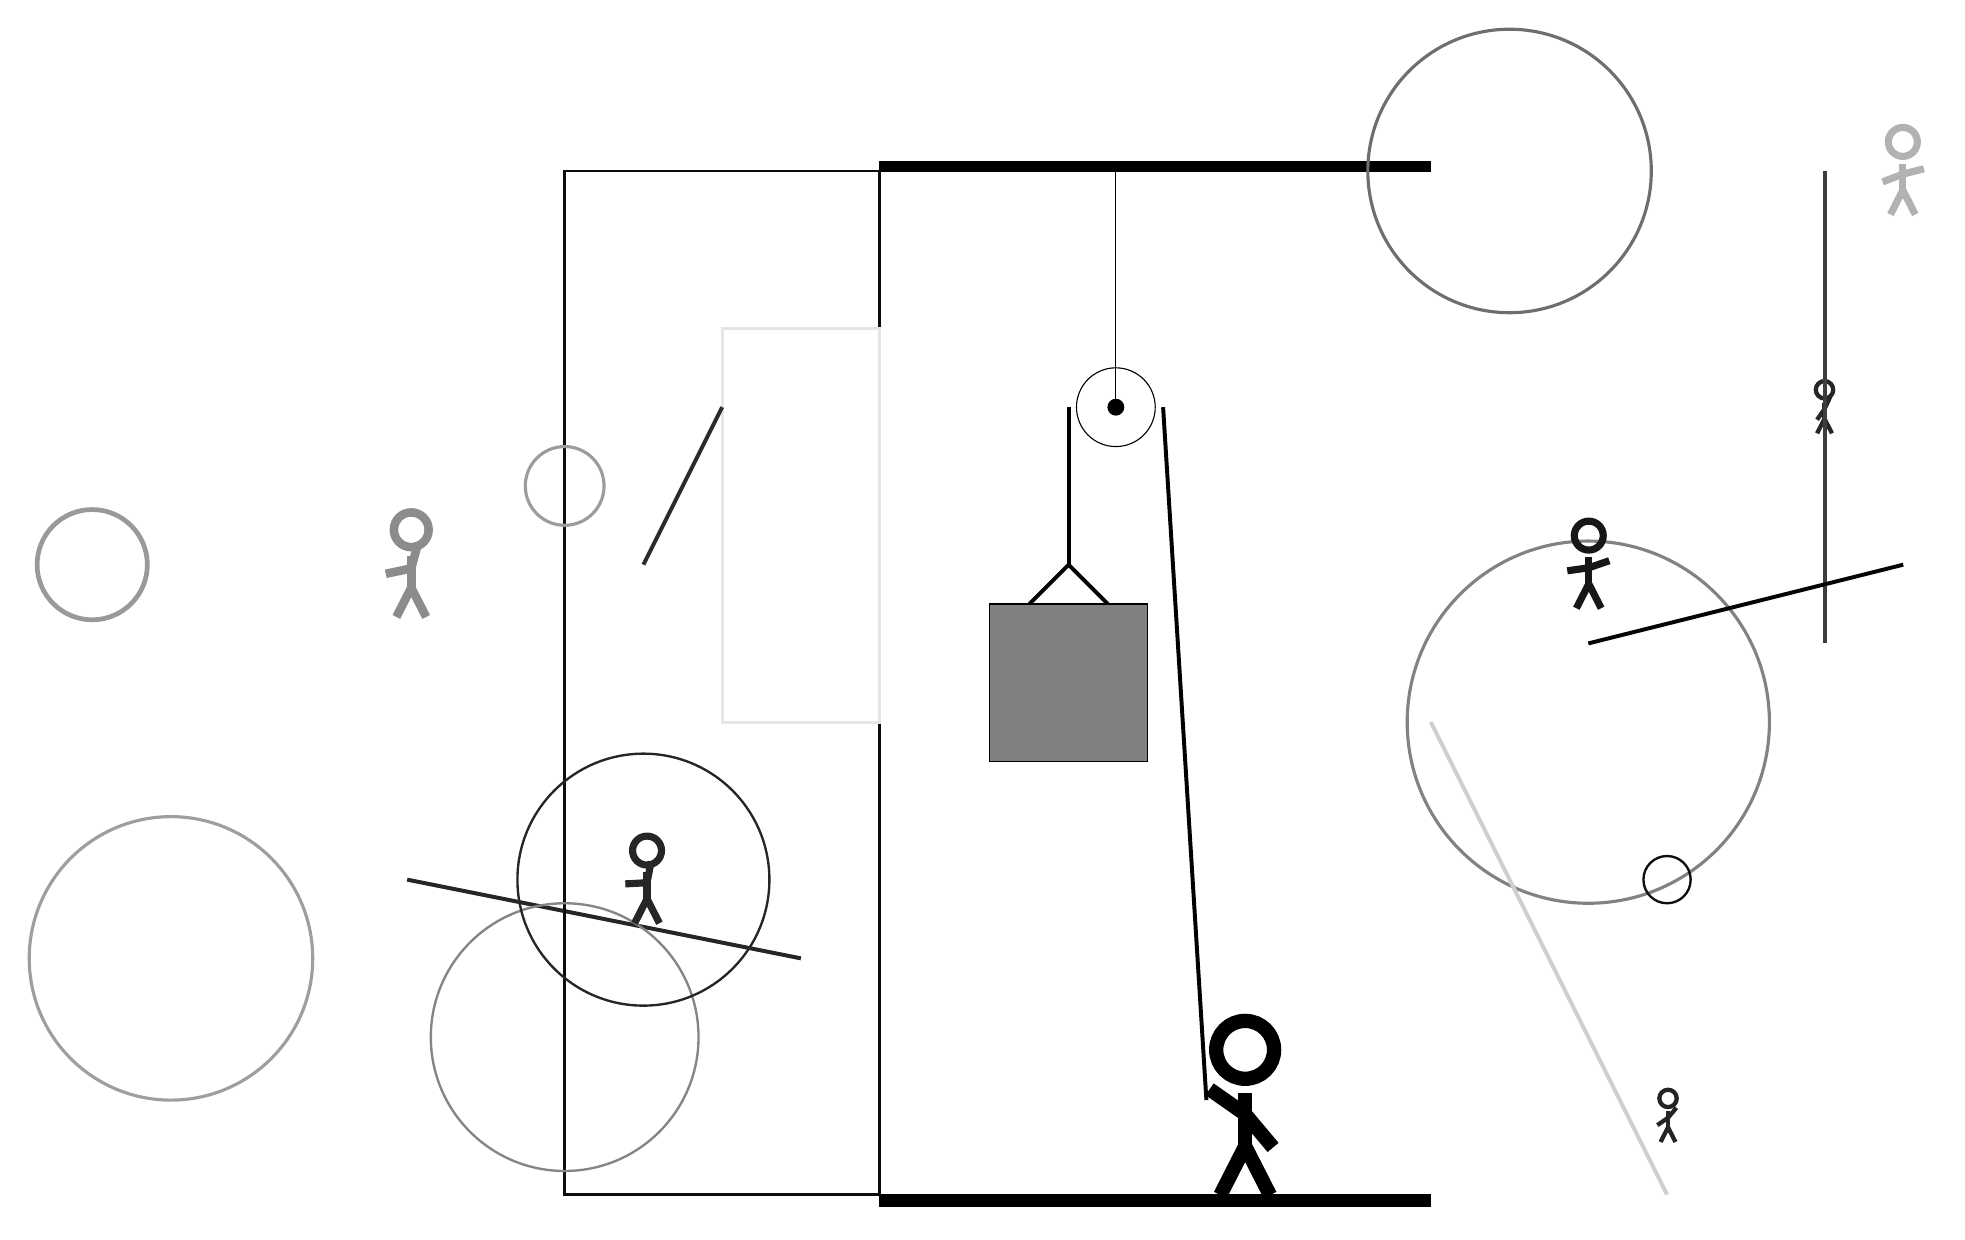
\begin{tikzpicture}
		%%%%% START %%%%%
		
		\draw[fill=black] (-2, 10) rectangle (5, 10.125);
		
		\draw (1, 7) circle (0.5);
		\draw[fill=black] (1, 7) circle (0.1);
		\draw (1, 10) -- (1, 7);
		
		\draw[line width=0.5mm] (-0.1, 4.5) -- (0.4, 5.0) -- (0.9, 4.5);
		\draw[fill=black!50] (-0.6, 4.5) rectangle (1.4, 2.5);
		
		\draw[line width=0.5mm, color=black!85](-3, 0) -- (-8, 1);
		
		\draw[line width=0.3mm, color=black!95] (-2, 10) rectangle (-6, -3);
		\node[line width=0.3mm, color=black!86] at (8, -2) {\Strichmaxerl[3][35][50]};
		\draw [line width=0.4mm, color=black!38](-11, 0) circle (1.8);
		
		\draw[line width=0.4mm, color=black!10] (-2, 8) rectangle (-4, 3);
		\node[line width=0.4mm, color=black!85] at (10, 7) {\Strichmaxerl[3][55][65]};
		\draw[line width=0.5mm, color=black!83](-4, 7) -- (-5, 5);
		
		\draw [line width=0.4mm, color=black!49](7, 3) circle (2.3);
		\draw [line width=0.3mm, color=black!48](-6, -1) circle (1.7);
		
		\draw[line width=0.5mm, color=black!19](5, 3) -- (8, -3);
		
		\draw [line width=0.6mm, color=black!40](-12, 5) circle (0.7);
		
		\draw [line width=0.4mm, color=black!57](6, 10) circle (1.8);
		\draw[line width=0.5mm, color=black!76](10, 10) -- (10, 4);
		
		\node[line width=0.6mm, color=black!85] at (-5, 1) {\Strichmaxerl[5][3][79]};
		\node[line width=0.2mm, color=black!30] at (11, 10) {\Strichmaxerl[5][21][14]};
		\node[line width=0.4mm, color=black!91] at (7, 5) {\Strichmaxerl[5][8][19]};
		
		\node[line width=0.7mm, color=black!45] at (-8, 5) {\Strichmaxerl[6][12][75]};
		
		\draw [line width=0.3mm, color=black!94](8, 1) circle (0.3);
		\draw [line width=0.4mm, color=black!39](-6, 6) circle (0.5);
		\draw[line width=0.5mm, color=black!98](7, 4) -- (11, 5);
		\draw [line width=0.3mm, color=black!85](-5, 1) circle (1.6);
		
		\draw[line width=0.5mm] (0.4, 7) -- (0.4, 5.0);
		\centerarc[line width=0.5mm](1, 7)(0:180:0.6);
		\draw[line width=0.5mm](1.6, 7) -- (2.15, -1.8);
		
		\node at (2.6, -1.9) {\Strichmaxerl[10][-35][-50]};
		
		\draw[fill=black] (-2, -3) rectangle (5, -3.15);
		
		%%%%% END %%%%%
	\end{tikzpicture}
\end{document}